%\documentclass[letter]{article}
\documentclass[10pt]{article}
\title{Nonlinear Macroeconomic Effects in Commercial Real Estate Vacancy Forecast Models}
%\author{CoStar}
\author{Michael Taylor}
\date{The American Real Estate Society $|$ ARES April 2019}
%\date{}
\usepackage{amsmath}
\usepackage{verbatim}
\usepackage{booktabs}
\usepackage{multirow}
\usepackage{graphicx}

\begin{document}
\maketitle
%\tableofcontents
%\pagestyle{headings}

%\begin{center}
%\section*{PPR Forecast Model Summary}
%\end{center}

\begin{abstract}
Commercial real estate forecast models are traditionally a function of macroeconomic data and other commercial real estate data.  The independent variables in these models are typically either not transformed, transformed using differences or growth rates, or transformed using logs or log differences.  These models tend to perform well, especially during periods of relatively stable economic growth.  But these models can underperform during periods of very strong or very weak economic conditions.  In reality, this is because the relationship between the economy and commercial real estate is complex and nonlinear.  This paper examines several methods of incorporating this nonlinear relationship into commercial real estate vacancy forecast models, such as by using nonlinear transformations of economic variables and by incorporating a recession dummy variable, and evaluates their performance.  We find that these methods do tend to add information to the forecast model; and that the probability of recession by metro$-$a nonlinear transformation of employment$-$performs particularly well.
\end{abstract}

\section*{Introduction}
Commercial real estate forecast models are traditionally a function of macroeconomic data and other commercial real estate data.  The independent variables in these models are typically either not transformed, transformed using differences or growth rates, or transformed using logs or log differences (see Table \ref{trans}).  These transformations result in relatively linear effects between changes in independent variables and changes in dependent variables.

\begin{table}[h]
\caption{Typical Independent Variable Transformations} \label{trans}
\begin{center}
\begin{tabular}{l l}
Equation & Description \\ \midrule
$X_t$ & No transformation \\
$X_t-X_{t-k}$ & First difference \\
$X_t/X_{t-k}-1$ & Percentage change or growth rate \\
$ln(X_t)$ & Natural logarithm \\
$ln(X_t)-ln(X_{t-k})$ & First difference of natural logarithm \\
\midrule
\end{tabular}
\end{center}
\label{default}
\end{table}%

For example, if a $2\%$ increase in $x$ leads to a $1\%$ increase in $y$ and a $4\%$ increase in $x$ leads to a 2\% increase in $y$, then a $-6\%$ change in $x$ will lead to a $-3\%$ change in $y$; at least as far as the model is concerned.  What we find in the real world, however, is the while these linear relationships tend to hold during normal periods of relatively stable economic growth, they can sometimes underperform during periods of very strong or very weak economic conditions.  In our example above, then, we might expect a $-6\%$ change in $x$ to actually correspond to a change of $-4\%$ in $y$ when looking at actual data.

Another way of framing this is that the model error or model residual will tend to be further from zero during periods of macroeconomic stress or exuberance.  This can be an issue for model users, who are often trying to capture those very periods of when the economy and commercial real estate are performing under extreme conditions.

\section*{Data}

The commercial real estate data in this paper are sourced from CoStar's vast database of surveyed properties in the United States.  The includes data for 4.5 million properties.  The data fields that we use in our analysis are vacancy and stock.

The macroeconomic data used are total non-farm payroll employment sourced from the BLS and business cycle (recession/expansion) dates sourced from the National Bureau of Economic Research (NBER).

Our analysis includes data from 42 metropolitan areas in which CoStar has been collecting data since at least 2000; as well as for the 4 major commercial property types of apartment, industrial, office, and retail.

\section*{Nonlinear Transformations}
In reality, the relationship between the economy and commercial real estate is complex and nonlinear.  During certain time periods, however, linear relationships may do a good job of approximating this complex relationship.  During other periods, as mentioned above, such as those of very strong or very weak economic conditions, we may need to use nonlinear transformations in order to better capture this complex relationship.  

\begin{table}[h]
\caption{Nonlinear Independent Variable Transformations} \label{newtrans}
\begin{center}
\begin{tabular}{l l}
Equation & Description \\ \midrule
$X^2_t$ & Squared \\
$X^3_t$ & Cubed \\
$P(R_t)$ & Probability of recession \\
$P(R_{t,i})$ & Probability of recession by metro \\
$R_t$ & Recession dummy \\
\midrule
\end{tabular}
\end{center}
\label{default}
\end{table}%

Table \ref{newtrans} lists several nonlinear independent variable transformations that we will later use to try to better incorporate the relationship between the economy and commercial real estate in our forecast models.  $X^2$ and $X^3$ are fairly straightforward baseline nonlinear transformations, and they will take a macroeconomic variable and square it or cube it, respectively.  These variables will amplify the effect of changes in $X$ on $Y$ as the values of $X$ get larger and larger or smaller and smaller.  

$R_t$ is a dummy variable that equals 1 if there is a recession and 0 if there is not a recession in a given quarter.  Whether or not the U.S. economy is in recession is determined by the NBER, who uses their industry accepted method of dating the peaks and troughs of business cycles.

$P(R_t)$ models the probability of $R_t$ as a function of the first difference of log national employment using a binary logistic regression.  And lastly, $P(R_{t,i})$ has the same model as $P(R_t)$ but uses metro employment as the independent variable instead of national employment.  Equation \ref{genform} shows the model specification of $P(R_t)$, which uses a binary logistic regression.
\begin{equation} \label{genform}
\begin{aligned}
& \text{P}(R_t) = \Lambda \left( X\beta + \varepsilon \right) 
& \text{where } \Lambda(x) = \frac{\text{e}^x}{1+\text{e}^x}
\end{aligned}
\end{equation}

Where P$(R_t)$ is the probability of $R_t$, $X$ is the independent variable matrix including first difference log national employment, $\beta$ is the vector of coefficient estimates, $\varepsilon$ is the error term, and $\Lambda(x)$ is logistic cumulative distribution function.

\begin{table}[h]
\caption{Estimation Results for Recession Model} \label{reg:rec}
\begin{center}
\begin{tabular}{l c}
{} & Coefficient \\ \midrule
\multirow{2}*{Constant} & -2.5014 \\
{} & (-3.24) \\
\multirow{2}*{Employment} & -871.0072 \\
{} & (-3.91) \\
\midrule
N & 137 \\
Pseudo R$^2$ & 0.7555 \\
Sensitivity & 0.8889 \\
Specificity & 0.9748 \\
AUC & 0.9860 \\
\midrule
\multicolumn{2}{l}{The $t$ statistics are shown} \\
\multicolumn{2}{l}{in parenthesis.}
\end{tabular}
\end{center}
\label{default}
\end{table}%

Table \ref{reg:rec} shows the estimation results of the recession model.  The in-sample results show that the model is highly predictive of recessions.  The sensitivity of the model is 88.89\%.  Sensitivity is the probability of the model predicting a recession given that a recession has occurred, i.e.~P$(+|R_t=1)$, where $+$ indicates that the predicted P$(R_t)\ge0.5$.  In other words, in 89\% of cases where there was a recession in a given quarter, the model had a predicted value greater than 0.5.

Additionally, the model has a specificity of 97.48\%.  Specificity is the somewhat opposite of sensitivity; it is the P$(-|R_t=0)$, where $-$ indicates that predicted P$(R_t)<0.5$.  This means that in 97\% of cases where there was not a recession in a given quarter, the model had a predict value less than 0.5.

Combining both sensitivity and specificity, the ROC curve is a plot of sensitivity vs.~1 $-$ specificity.  The area under the ROC curve (AUC) is often used as a measure of fit for binary choice models, with a value of 1 indicating a perfect fit and a value of 0.5 indicating a model no better than chance.  The model has an AUC of 0.9860, again indicating a strong fit.

\begin{figure}[h]
\begin{center}
\caption{Recession Model Fitted Values} \label{fig:rec}
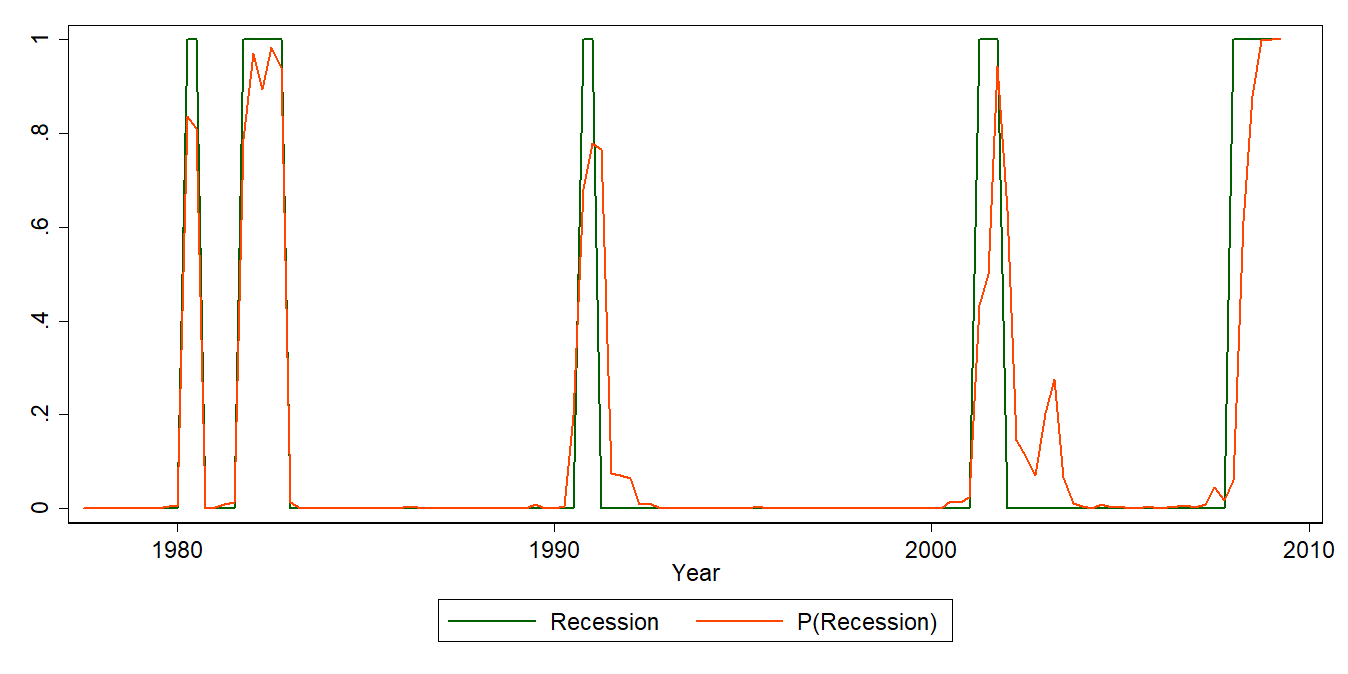
\includegraphics[scale=0.22]{rec-fitted-6.png}
\end{center}
\end{figure}

Figure \ref{fig:rec} shows periods of recession over the last several decades as well as the fitted values from the recession model.  In addition to the model testing results, it is also visually clear that the recession model delineates well between periods of economic recession and expansion.

Taking a step back, the above model is essentially a nonlinear transformation of the employment variable calibrated to whether there is a recession or not.  Using the predicted values from this model, it allows us to include additional information in our forecast model that is contained in the extreme values of employment, as a recession is only indicated when employment growth reaches a low enough threshold.  And given that this recession model uses employment as its only independent variable, its fitted values could easily be incorporated into a vacancy forecast model that already includes employment.

\section*{Modeling Vacancy}
Up until now we've discussed in general how to incorporate additional information into models using various nonlinear transformations.  In this section, we will apply these to the specific example of a commercial real estate vacancy forecast model. The baseline model specification for vacancy can be seen in Equation \ref{eq:baseline}.
\begin{equation} \label{eq:baseline}
\Delta V_t = \beta_0 + \beta_1 \Delta E_{t-1} + \beta_2 \Delta S_{t-1} + \varepsilon
\end{equation}

Where $V_t$ is first difference log vacancy, $\Delta E_{t-1}$ is lagged second difference log employment, $\Delta S_{t-1}$ is lagged first difference log stock, and $\varepsilon$ is the error term.  Equation \ref{eq:baseline} is estimated using ordinary least squares, and $\beta_0 \dots \beta_n$ represent the coefficient estimates.

In a previous analysis, we established that vacancy level is co-integrated with changes in employment.  Thus, vacancy change is modeled here as a function of second order changes in employment.  Note that we omit the co-integrating equation from the analysis in this paper for the sake of simplicity in evaluating models, but we would include it in a final vacancy forecast model.

\begin{table}[h]
\caption{Additional Independent Variables} \label{table:vars}
\begin{center}
\begin{tabular}{l l}
Equation & Description \\ \midrule
$(\Delta E_{t-1})^2$ & Squared Employment Growth \\
$(\Delta E_{t-1})^3$ & Cubed Employment Growth \\
$R_t$ & Recession dummy \\
$P(R_t)$ & Probability of recession \\
$P(R_{t,i})$ & Probability of recession by metro \\
\midrule
\end{tabular}
\end{center}
\label{default}
\end{table}%

Table \ref{table:vars} shows each of 5 variables that will be added individually to Equation \ref{eq:baseline} with a coefficient estimate of $\beta_3$, in an attempt to improve on the baseline results, and all 6 resulting model specifications will be compared subsequently.  Note that $(\Delta E_{t-1})^2$ and $(\Delta E_{t-1})^3$ represent a squaring and cubing, respectively, of the lagged second difference log employment term in Equation \ref{eq:baseline}.  The additional recession variables are the same as listed above in Table \ref{newtrans} and in the discussion following it.

{
\begin{table}[h]
\begin{center}
\caption{Estimation Results for Vacancy Models} \label{reg:all}
\begin{tabular}{l c c c c c c}
{} & Baseline & $(\Delta E_{t-1})^2$ & $(\Delta E_{t-1})^3$ & $P(R_t)$ & $P(R_{t,i})$ & $R_t$ \\ \midrule
\multirow{2}*{Constant} & -0.0114 & -0.0146 & -0.0111 & -0.0157 & -0.0164 & -0.0136 \\
{} & (-14.18) & (-17.29) & (-13.85) & (-18.88) & (-19.70) & (-17.02) \\
\multirow{2}*{$\Delta E_{t-1}$} & -1.2024 & -1.1689 & -1.4600 & -0.6590 & -0.6208 & -0.8823 \\
{} & (-24.23) & (-23.66) & (-19.90) & (-11.29) & (-10.73) & (-17.00) \\
\multirow{2}*{$\Delta S_{t-1}$} & 0.8435 & 0.8378 & 0.8251 & 0.7918 & 0.7797 & 0.7190 \\
{} & (15.98) & (15.98) & (15.61) & (15.19) & (14.99) & (13.72) \\
Additional & & 27.5448 & 474.1052 & 0.0344 & 0.0343 & 0.0294 \\
Variable & & (11.76) & (4.76) & (17.08) & (18.71) & (18.32) \\
\midrule {N} & 10,579 & 10,579 & 10,579 & 10,579 & 10,579 & 10,579 \\
{R$^2$} & {0.1071} & 0.1178 & 0.1096 & 0.1319 & \bf{0.1387} & 0.1367 \\
{MAE} & {0.03493} & 0.03442 & 0.03491 & 0.03420 & \bf{0.03415} & 0.03428 \\
{RMSE} & {0.05055} & 0.05022 & 0.05050 & 0.04986 & \bf{0.04972} & 0.04976 \\
{VIF} & 1.12 & 1.08 & 1.96 & 1.43 & 1.41 & 1.20 \\
\midrule
\multicolumn{7}{l}{The $t$ statistics are shown in parentheses. The highest R$^2$ and lowest} \\
\multicolumn{7}{l}{MAE and RMSE values are highlighted in bold.}
\end{tabular}
\end{center}
\end{table}
}

Table \ref{reg:all} shows the in-sample estimation results from the 6 model specifications described above.  The name of the model (either baseline or the additional variable added) labels the columns.  And in the first column, in each row are the variables included in the regression.  In the table are their parameter estimates and $t$ statistics; as well as select goodness of fit measures and the variance inflation factor (VIF) test.  The model estimation is done using a fixed effects panel regression that includes 42 metros, 4 property types, and an average of 63 observations per group$-$for a total of 10,579 observations used in the model.

The in-sample results indicate that every model with an additional variable is an improvement over the baseline model.  This is more or less to be expected with the in-sample results, but does demonstrate that none of that additional variables are wildly problematic.  The strongest model is with $P(R_{t,i})$, which is the predicted probability of recession by metro variable.  It has the highest R$^2$ and the lowest mean absolute error (MAE) and root mean squared error (RMSE).

The coefficients for the constant and $\Delta S_{t-1}$ are largely the same relative to the baseline model.  But the coefficients for $\Delta E_{t-1}$ do change depending on which additional variable is added$-$particularly for the models with $P(R_t)$ and $P(R_{t,i})$ added.  For these, the coefficient goes from around -1.2 in the baseline model to around -0.6, falling by around half.  There doesn't appear to be any issue with this, but it does indicate that the additional of predicted recession probabilities based on a model that includes employment, is taking away some of the influence of the employment growth variable in the baseline model. Given the strong relationship between several of the independent variables, the VIF was calculated to test for multicollinearity.  Typically, a VIF greater than 5 indicates multicollinearity$-$all vacancy models have a VIF less than 5, indicating that there is no multicollinearity.

\begin{figure}[h]
\begin{center}
\caption{Chicago Industrial In-Sample Fitted Values} \label{fig:chic-in}
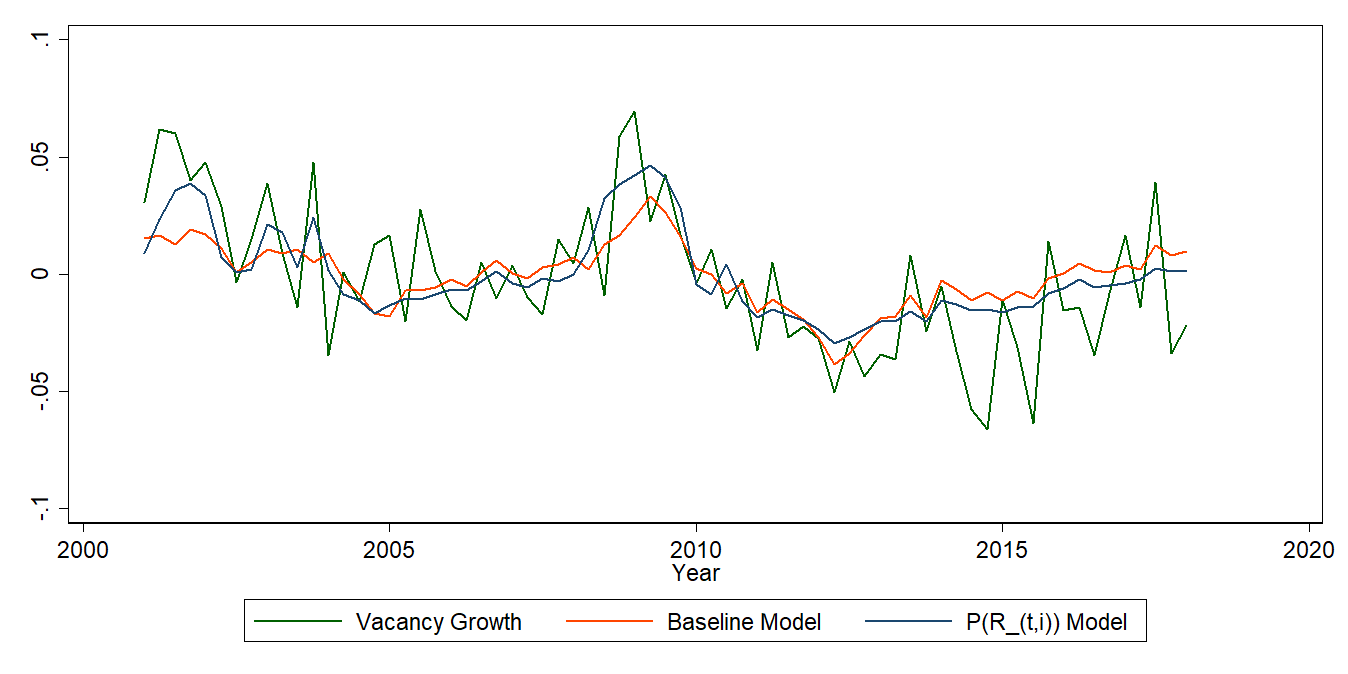
\includegraphics[scale=0.22]{chicind-insample-3.png}
\end{center}
\end{figure}

Figure \ref{fig:chic-in} shows the vacancy growth and in-sample fitted values of selected models for Chicago industrial.  The two models shown are the baseline and the highest performing $P(R_{t,i})$ model.  Note that for readability the probability of recession is not shown on the figure, but the probabilities are high during 2001 and 2009 approximately.  

Comparing the fitted values for the two models, both follow similar trends and line up closely with the actual vacancy growth.  But upon closer inspection, we see that during periods of economic stress such as 2001 and 2009, the $P(R_{t,i})$ model fitted values are higher then the baseline's.  And during period of stable economic growth such as 2014-2018, the $P(R_{t,i})$ model fitted values are either lower or very close to the baseline's.  In both cases, the $P(R_{t,i})$ model fitted values are on average closer to the actual vacancy growth values.

\begin{figure}[h]
\begin{center}
\caption{New York Office In-Sample Fitted Values} \label{fig:newy-in}
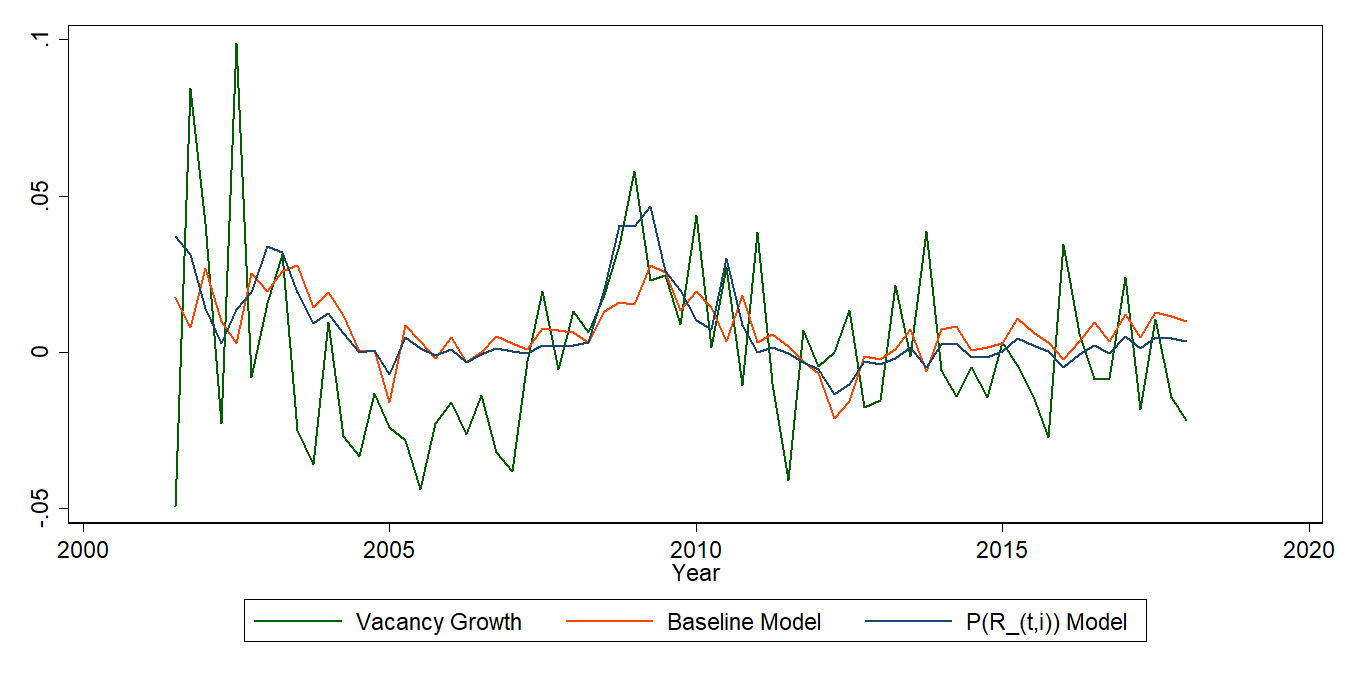
\includegraphics[scale=0.22]{newyoff-insample-2.png}
\end{center}
\end{figure}

Figure \ref{fig:newy-in} similarly shows the vacancy growth and in-sample fitted values for New York office; and compares the baseline and the $P(R_{t,i})$ models.  The results of New York office are similar to those of Chicago industrial.  The $P(R_{t,i})$ model fitted values are more sensitive to the business cycle$-$higher during periods of economic stress (2001, 2009) and lower or similar during more stable economic periods (2003-2006, 2014-2018).  These results align with our expectations, and further affirm that the $P(R_{t,i})$ model does a better job than the baseline model of capturing the nonlinear relationship between the economy and commercial real estate vacancy.

\section*{Out-of-Sample Results}

While the in-sample results are promising, our ultimate goal is to determine if the addition of nonlinear variables will improve the forecasting results of the vacancy model.  To test this, the following section will look at the results of 2 different 5-year out-of-sample forecast runs for the 6 models above.  The first will fit the model through 2007Q4 and generate model predictions over the period 2008Q1 through 2012Q4 and compare the model predictions to actuals.  And the second will fit the model through 2012Q4, predict from 2013Q1 through 2017Q4, and compare to actuals.

{
\begin{table}[h]
\caption{Out-of-Sample Results (2008Q1-2012Q4)} \label{reg:os1}
\begin{center}
\begin{tabular}{l c c c c c c}
{} & Baseline & $(\Delta E_{t-1})^2$ & $(\Delta E_{t-1})^3$ & $P(R_t)$ & $P(R_{t,i})$ & $R_t$ \\
\midrule
{N} & 3,691 & 3,691 & 3,691 & 3,691 & 3,691 & 3,691 \\
{MAE} & {0.03422} & 0.03489 & 0.03494 & {0.03605} & \bf{0.03347} & 0.03495 \\
{RMSE} & {0.04589} & 0.04674 & 0.04545 & {0.04771} & \bf{0.04479} & 0.04641 \\
\midrule
\multicolumn{7}{l}{The lowest MAE and RMSE values are highlighted in bold.}
\end{tabular}
\end{center}
\end{table}
}

Table \ref{reg:os1} shows the results of the first out-of-sample test that fits the model through 2007Q4 and predicts and compares to actuals over the period 2008Q1 through 2012Q4.  The model is calibrated on 3,691 observations and predicts and compares to actuals for 3,360 observations.  Also note that this out of sample period includes a national recession for 6 quarters from 2008Q1 through 2009Q2.

The out of sample results agree with the in sample results concerning which of the 6 is the strongest model$-$again the model containing $P(R_{t,i})$ outperforms the other 5 models.  At 0.03347 and 0.04479, the MAE and RMSE respectively of the $P(R_{t,i})$ model is lower than the baseline model and much lower than some of the other models.  

{
\begin{table}[h]
\caption{Out-of-Sample Results (2013Q1-2017Q4)} \label{reg:os2}
\begin{center}
\begin{tabular}{l c c c c c c}
{} & Baseline & $(\Delta E_{t-1})^2$ & $(\Delta E_{t-1})^3$ & $P(R_t)$ & $P(R_{t,i})$ & $R_t$ \\
\midrule
{N} & 7,051 & 7,051 & 7,051 & 7,051 & 7,051 & 7,051 \\
{MAE} & {0.03948} & 0.03859 & 0.03947 & {0.03795} & \bf{0.03757} & 0.03829 \\
{RMSE} & {0.05412} & 0.05332 & {0.05412} & {0.05274} & \bf{0.05249} & 0.05302 \\
\midrule
\multicolumn{7}{l}{The lowest MAE and RMSE values are highlighted in bold.}
\end{tabular}
\end{center}
\end{table}
}

Table \ref{reg:os2} shows the results of the second out-of-sample test that fits the model through 20012Q4 and predicts and compares to actuals over the period 2013Q1 through 2017Q4.  The model is calibrated on 7,051 observations and predicts and compares to actuals for 3,360 observations.  This period does not include a recession.

Once again, the $P(R_{t,i})$ model has the lowest MAE at 0.03757 and RMSE at 0.05249.  This result lines up well with the first out-of-sample test and with the in-sample results.  Given the results of both of the out-of-sample tests covering recessionary and expansionary periods, it is clear that the model containing the additional $P(R_{t,i})$ variable has the strongest fit and the best forecasting performance.

\section*{Forecasting Implications}

Next, we look at the impact of the $P(R_{t,i})$ model on forecasting and compare it to the forecasts of our baseline model.  The $P(R_{t,i})$ model includes the additional independent variable of probability of recession by metro; and the goal in this section is to visually inspect how strong the impacts of the additional recession variable are on the vacancy forecast.

\begin{figure}[h]
\begin{center}
\caption{New York Office Base Case Forecast} \label{fig:newy-fc-1}
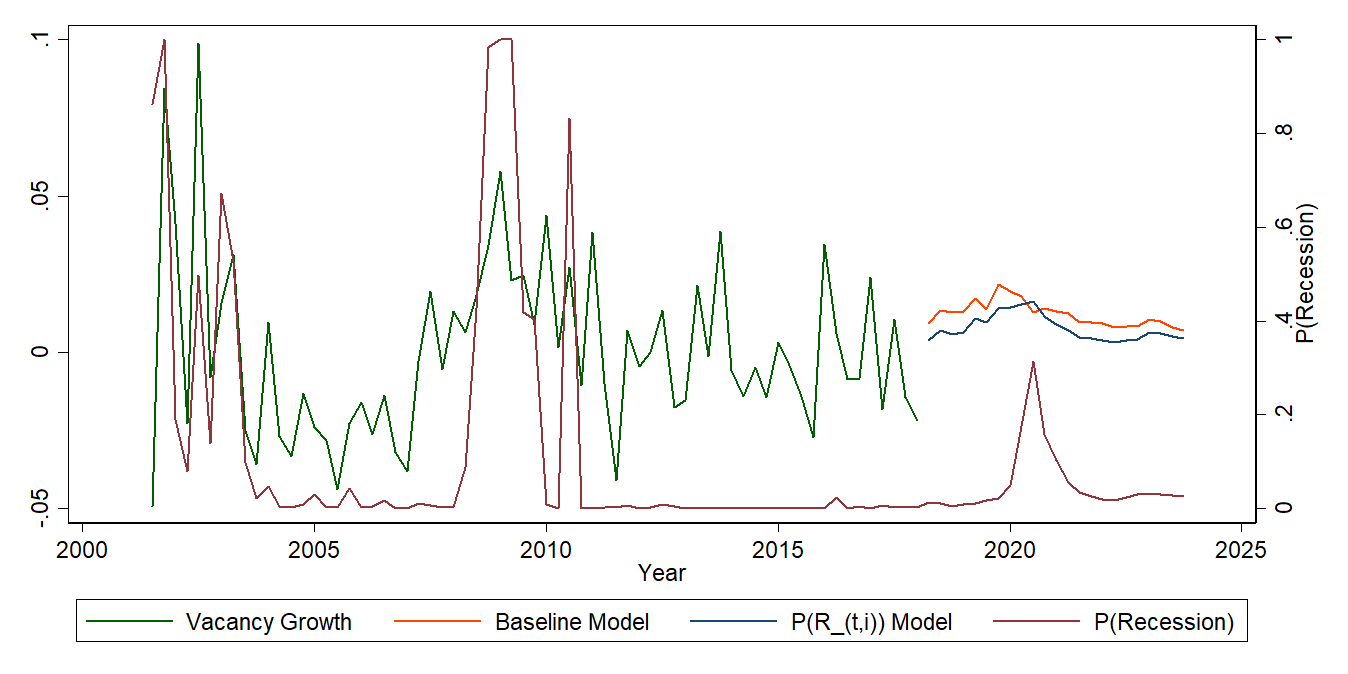
\includegraphics[scale=0.22]{newyoff-forecast-simid1-2.png}
\end{center}
\end{figure}

Figure \ref{fig:newy-fc-1} shows a vacancy growth forecast for New York office under a base case economic forecast scenario.  The figure shows two forecasts: one for the baseline model and one for the $P(R_{t,i})$ model with an additional probability of recession by metro independent variable.  Also, the probability of recession by metro is shown on the right y-axis.  The probability peaks at approximately 30\% in the forecast, as the base case scenario contains a slowdown in economic growth in 2020.

Comparing the two forecasts, it is clear that they are quite similar under a base case economic forecast scenario.  The baseline model is slightly higher throughout the forecast.  This reflects that the $P(R_{t,i})$ model ``knows'' that there isn't a recession in the forecast, and thus has a correspondingly lower (and better) vacancy forecast.  Note that the two forecasts do cross over each other for a quarter when the probability of recession is spikes to 30\%.  And while it doesn't indicate a full on recession, it does indicate a slight chance of one, and thus the vacancy forecast is slightly higher.  Overall, the $P(R_{t,i})$ model is slightly more cyclical, even under base case economic conditions.

\begin{figure}[h]
\begin{center}
\caption{New York Office Recession Forecast} \label{fig:newy-fc-5}
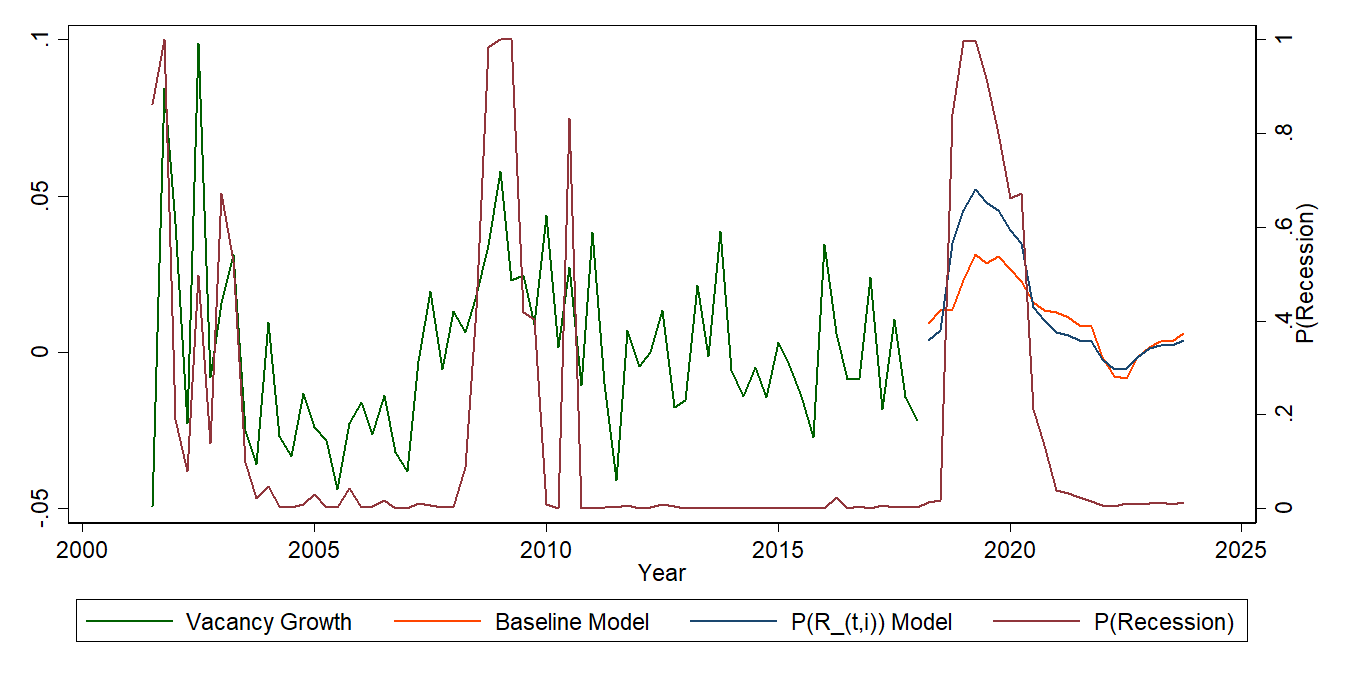
\includegraphics[scale=0.22]{newyoff-forecast-simid5-2.png}
\end{center}
\end{figure}

Figure \ref{fig:newy-fc-5} shows a vacancy growth forecast for New York office under a recession economic forecast scenario.  Note that compared to the previous figure, this one has a probably of recession forecast that peaks at 100\% and remains above 50\% for several quarters; as the recession scenario contains negative employment growth in 2019 and 2020.

Comparing the impact of the recession on the two vacancy forecasts, both see an increase in vacancy growth during the recession, though there is more differentiation between the two forecasts than under the base case economic scenario.  The $P(R_{t,i})$ model has a much higher increase in vacancy growth than the baseline model$-$because the $P(R_{t,i})$ model explicitly factors in the recession in this scenario.  Note that in Figure \ref{fig:newy-fc-1} the $P(R_{t,i})$ vacancy forecast is \emph{lower} than baseline and in Figure \ref{fig:newy-fc-5} the $P(R_{t,i})$ vacancy forecast is \emph{higher} than baseline$-$this is the expected result, and will contribute well to more differentiation between the vacancy forecasts under various economic scenarios.

\section*{Conclusion}
In this paper, we examined a baseline vacancy forecast model and compared it to five other models each with an additional independent variable.  We examined both in-sample and out-of-sample results.  We found that while the baseline model performed quite well under these various circumstances, the addition of nonlinearly transformed variables added additional information to and improved the fit of our models.  Even though employment was already a factor in our vacancy forecast model, the addition of the fitted values from a recession model using metro employment as its independent variable improved the fit of our vacancy model the most, demonstrating that there was additional information in the employment variable that we were able to add to our vacancy model by nonlinearly transforming it.  In other words, by modeling a recession as a function of employment, a variable which was already included in our vacancy model, and incorporating its predicted values, we were able to generate a better forecast without using any additional exogenous variables.

These findings are important for several reasons: 1) they underscore the importance that the real world is complex and nonlinear and that models attempting to approximate the real world could benefit from looking at nonlinear transformations of variables, and 2) they demonstrate a practical method to better model commercial real estate over recessionary and expansionary periods in forecast models.

Future research would certainly investigate adding nonlinear macroeconomic effects to other commercial real estate models such as cap rate.  It might also look at additional nonlinear transformations of the employment variable; or additional variables incorporated into the recession model, such as interest rates, though this would increase the number of exogenous variables that require an economic forecast.  It might also investigate separate property types or separate metro models to determine if these are more or less sensitive to recessions than others.






\end{document}

